\documentclass{beamer}
\usetheme{AnnArbor}

\title{Corporate default prediction}
\subtitle{Statistics for Data science - AEM University of Brescia}
\author{Mateusz Dadej}
\date{\today}

\begin{document}

\begin{frame}
\titlepage
\end{frame}

\begin{frame}{Research questions}
\begin{itemize}
\item What are the consequences of applying different resampling methods? Is the more complex the better?
\item What's the most efficient way to make a model of a corporate probability of default?
\end{itemize}
\end{frame}

\begin{frame}{Overview of data: Basic information}

\begin{itemize}
\item Data is sourced from Orbis - Private company database
\item Geographical location of companies are developed countries in Europe 
\item in period 2018-2020
\item observations were filtered with following criteria:
	\begin{itemize}
	\item Active, bancrupt or dissolved at time $t$
	\item With known value of some financial ratios at time $t-1$
	\item Standardised legal form: Private and public limited company
	\item Entity type: corporate
	\item known and higher than 5 number of employees at time $t-1$
	\end{itemize}

\end{itemize}

\end{frame}

\begin{frame}{Overview of data: descriptive statistics}

% geographical distribution
% number of NAs
% number of bancruptcies

\end{frame}

\begin{frame}{Data preprocessing}

\begin{itemize}
\item Variables with more than $25$\% not available values were dropped
\item Categorical variables were one-hot-encoded
\item NAs were imputed with the median of a given variable
\item Preprocessed dataset was split into training (80\%) and testing dataset 

\end{itemize}

\

For feature engineering, additional 20 new variables were introduced from initial 30, briefly:

\begin{itemize}
\item For some financial data like revenue, net proft, a relative change from previous year was introduced
\item Most of the original variables were a standard positions from finacial statement, thus financial ratios were introduced with some basic arithmetic operations.

\end{itemize} 

\end{frame}

\begin{frame}{Resampling methods}
Corporate default data is known to have a huge class imbalance problem. 

\

In order to adress the problem and investigate their modeling consequences, I further apply 3 resampling methods to the training dataset:

\begin{itemize}
\item Oversampling
\item Undersampling
\item Synthetic Minority Over-sampling Technique (SMOTE) [N. Chawla, et. al, 2002]
\end{itemize}

\

Further modeling workflow is done for datasets resampled with each of the methods above, in order to compere them.
\end{frame}

\begin{frame}{Applied models (1/3): Penalized logistic regression}

$$\min_{w,c} \frac{1-\rho}{2} \beta^{T}\beta + \rho ||\beta||_1 + C \sum_{i-1}^n \ln e^{-y_i(X_i^T \beta + c)}+1$$

Where:

\begin{itemize}
\item $\rho$ parameter regulating preference for l-2 or l-1 regularizaton
\item C paraemters regulating preference to regularization
\end{itemize}

\

Both of the parameters above were tuned with a grid search over corss validated results.


\end{frame}

\begin{frame}{Applied models (2/3): XGBoost - Gradient boosted decision trees}

\begin{itemize}
\item A workhorse ML model, based on an ensemble of decision trees [T. Chen, C. Guestrin, 2016].
\item Trained with a gradient boosting algorithm based on Friedman et al. 2000
\item The model is trained in a sequential way, each training round consists of function estimated from previous round and a newly trained one.
\item The objective function both tries to minimize log-loss and a regularization term, which penalizes number of leaves and a l-2 norm of leaf score
\item all in all, a complex model....

\item In herein project, the hyperparameters were tuned with random search.

\end{itemize}

\end{frame}

\begin{frame}{Applied models (3/3): Multilayer perceptron}

\begin{itemize}
\item Basic "vanilla" model of artificial neural networks
\item Estimates weights of "neurons" iteratively with backpropagation
\item Just like the previous model, can generalize non-linear patterns and has a regularization in a objective function
\end{itemize}

\

For this project, the hyperparameters were tuned with a random search.

\end{frame}

\begin{frame}{model fitness comparison - ROC}

\begin{center}
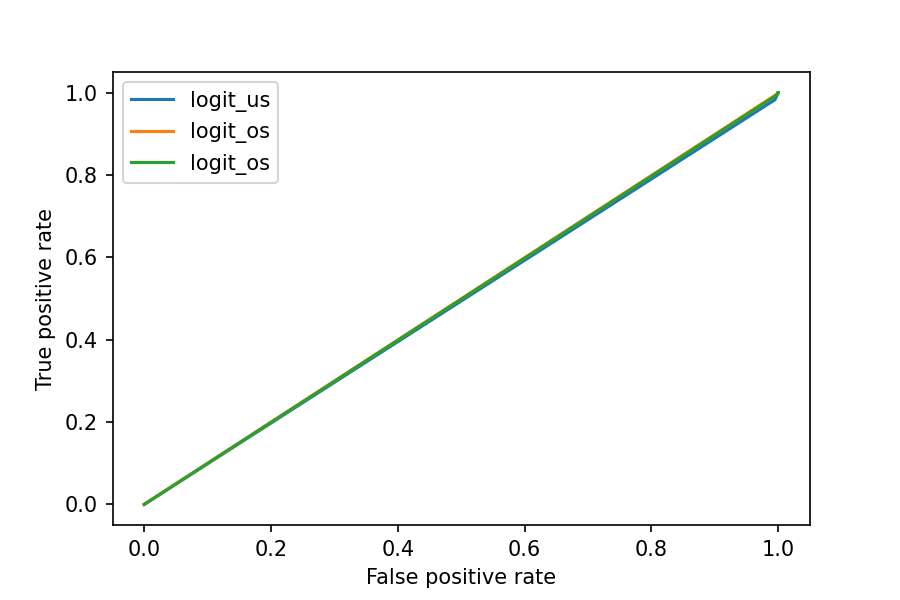
\includegraphics[scale=0.55]{img/log_roc.png}
\end{center}
\end{frame}

\begin{frame}{model fitness comparison - ROC}

\begin{center}
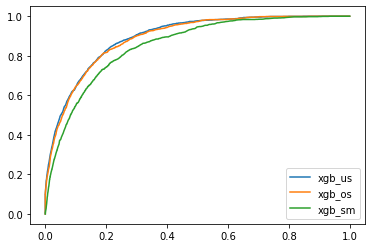
\includegraphics[scale=0.55]{img/xgb_roc.png}
\end{center}
\end{frame}

\begin{frame}{model fitness comparison - ROC}

\begin{center}
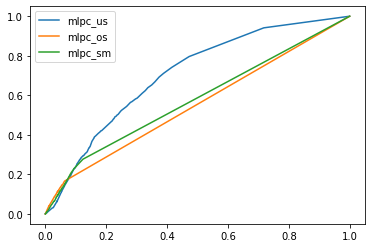
\includegraphics[scale=0.55]{img/mlpc_roc.png}
\end{center}
\end{frame}

\begin{frame}{References}

\begin{itemize}
\item N. V. Chawla, et. al, SMOTE: Synthetic Minority Over-sampling Technique, Journal of Artificial Intelligence Research 16, 2002
\item T. Chen, C. Guestrin, XGBoost: A Scalable Tree Boosting System, 2016
\item J. Friedman, T. Hastie, and R. Tibshirani. Additive logistic
regression: a statistical view of boosting. Annals of
Statistics
\end{itemize}
\end{frame}
\end{document}



